\documentclass[12pt,aspectratio=169]{beamer}

\usetheme{metropolis}

\definecolor{mDarkBrown}{HTML}{FF5722}
\definecolor{mDarkTeal}{HTML}{263238}
\definecolor{mLightBrown}{HTML}{FF5722}

\usepackage{booktabs}
\usepackage{graphicx}
\usepackage{hyphenat}
\usepackage{multirow}
\usepackage{nicefrac}
\usepackage[normalem]{ulem}

\usepackage{pifont}
\newcommand{\cmark}{\ding{51}}
\newcommand{\xmark}{\ding{55}}

\usepackage{minted}
\usemintedstyle{tango}
\newminted[bash]{bash}{%
    autogobble,
    bgcolor=mDarkTeal!10,
    linenos
}
\newminted[py3]{python}{%
    python3,
    autogobble,
    bgcolor=mDarkTeal!10,
    linenos
}
\newminted[sql]{sql}{%
    autogobble,
    bgcolor=mDarkTeal!10,
    linenos
}

\usepackage{polyglossia}
\setdefaultlanguage[variant=british]{english}
\usepackage[english=british]{csquotes}

\defaultfontfeatures{Ligatures=TeX}
\setmainfont{Lucida Sans OT}
\setsansfont[Scale=MatchLowercase]{Lucida Sans OT}
\setmonofont[Scale=MatchLowercase]{Lucida Console DK}

\usepackage{mathspec}
\setmathsfont(Digits,Latin,Greek)[Numbers={Lining,Proportional}]{Lucida Bright Math OT}

\newcommand{\mat}[1]{\ensuremath{\mathbf{#1}}}

\newcommand{\R}{\ensuremath{\mathbb{R}}}

\newcommand{\E}[1]{\ensuremath{\mathbb{E}\!\left[ #1 \right]}}
\newcommand{\V}[1]{\ensuremath{\mathbb{V}\!\left[ #1 \right]}}
\newcommand{\Prob}[1]{\ensuremath{\Pr\!\left( #1 \right)}}
\newcommand{\Normal}[2]{\ensuremath{\mathcal{N}\!\left( #1, #2 \right)}}
\newcommand{\simiid}{\ensuremath{\overset{\text{\tiny i.i.d.}}{\sim}}}

\DeclareMathOperator{\logit}{logit}

\author{Gianluca Campanella}
\date{}



\title{Introduction to dimensionality reduction}

\begin{document}

\maketitle

\begin{frame}{Contents}
    \tableofcontents[hideallsubsections]
\end{frame}

\section{Dimensionality reduction}

\begin{frame}{Dimensionality reduction}
    \only<1>{%
        \begin{block}{Idea}
            \begin{itemize}
                \item Identify correlated columns
                \item Replace them with a new column that `encapsulates' the
                      others
            \end{itemize}
        \end{block}
        \vfill
        \begin{block}{Example}
            \begin{itemize}
                \item \{ car, cat, truck, van \}
                \item[$\rightarrow$] \{ cat, vehicle \}
            \end{itemize}
        \end{block}}
    \only<2>{%
        \begin{block}{Why?}
            \begin{itemize}
                \item `True' dimensionality is lower
                \item Too many correlated variables $\rightarrow$ collinearity
                \item Difficult to visualise
            \end{itemize}
        \end{block}
        \vfill
        \begin{block}{How?}
            \begin{itemize}
                \item Project onto a \alert{lower\hyp{}dimensional} space\ldots
                \item \ldots while \alert{retaining (most of) some property}
            \end{itemize}
        \end{block}}
\end{frame}

\section{Manifold learning}

\begin{frame}{Multidimensional scaling (MDS)}
    \only<1>{%
        \begin{block}{Aim}\vspace{-0.5em}
            \begin{itemize}
                \item Project onto a lower\hyp{}dimensional space\ldots
                \item \ldots while \alert{retaining most of the distance
                      structure}
            \end{itemize}
        \end{block}
        \begin{block}{Method}\vspace{-0.5em}
            \begin{itemize}
                \item Input: dissimilarity matrix (not necessarily a metric)
                \item Find a `close' representation (squared loss)
            \end{itemize}
        \end{block}
        \vfill
        \begin{block}{Limitations}\vspace{-0.5em}
            \begin{itemize}
                \item Somewhat slow (numerical optimisation)
                \item Embeddings are not necessarily unique or `optimal'
            \end{itemize}
        \end{block}}
    \only<2>{%
        \begin{center}
            \vfill
            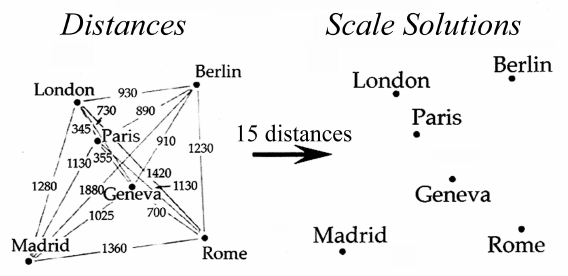
\includegraphics[width=0.8\textwidth]{figures/mds_cities_1} \\[\bigskipamount]
            {\scriptsize%
             From Cutting et al.\ (2013)}
            \vfill
        \end{center}}
    \only<3>{%
        \begin{center}
            \vfill
            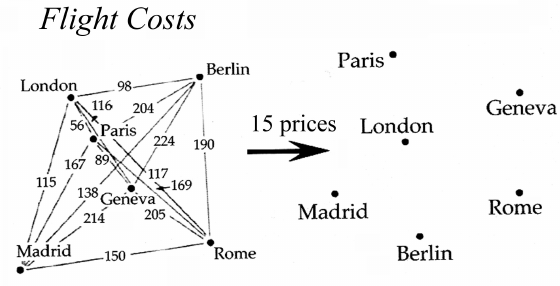
\includegraphics[width=0.8\textwidth]{figures/mds_cities_2} \\[\bigskipamount]
            {\scriptsize%
             From Cutting et al.\ (2013)}
            \vfill
        \end{center}}
\end{frame}

\section{PCA and PLS}

\begin{frame}{Principal component analysis (PCA)}
    \only<1>{%
        \begin{block}{Aim}\vspace{-0.5em}
            \begin{itemize}
                \item Project onto a lower\hyp{}dimensional space\ldots
                \item \ldots while \alert{retaining most of the correlation
                      structure}
            \end{itemize}
        \end{block}
        \begin{block}{Method}\vspace{-0.5em}
            \begin{itemize}
                \item Eigendecomposition of covariance/correlation matrix
                \item Typically using singular value decomposition (SVD)
            \end{itemize}
        \end{block}
        \vfill
        \begin{block}{Limitations}\vspace{-0.5em}
            \begin{itemize}
                \item \alert{Unsupervised} method
                      $\rightarrow$ outcome is disregarded
                \item PCs may not be explanatory of $\mat{Y}$
                      (noise\hyp{}driven)
            \end{itemize}
        \end{block}}
    \only<2>{%
        \begin{block}{Model}\vspace{-0.5em}
            \begin{itemize}
                \item Defined by the `direction' vectors $p_{i}$
                      (\alert{loadings})

                \item Loadings are oriented in such a way that the project data
                      $t_{i}$ (\alert{scores}) have maximum variance
            \end{itemize}
        \end{block}
        \vspace{-1em}
        \begin{center}
            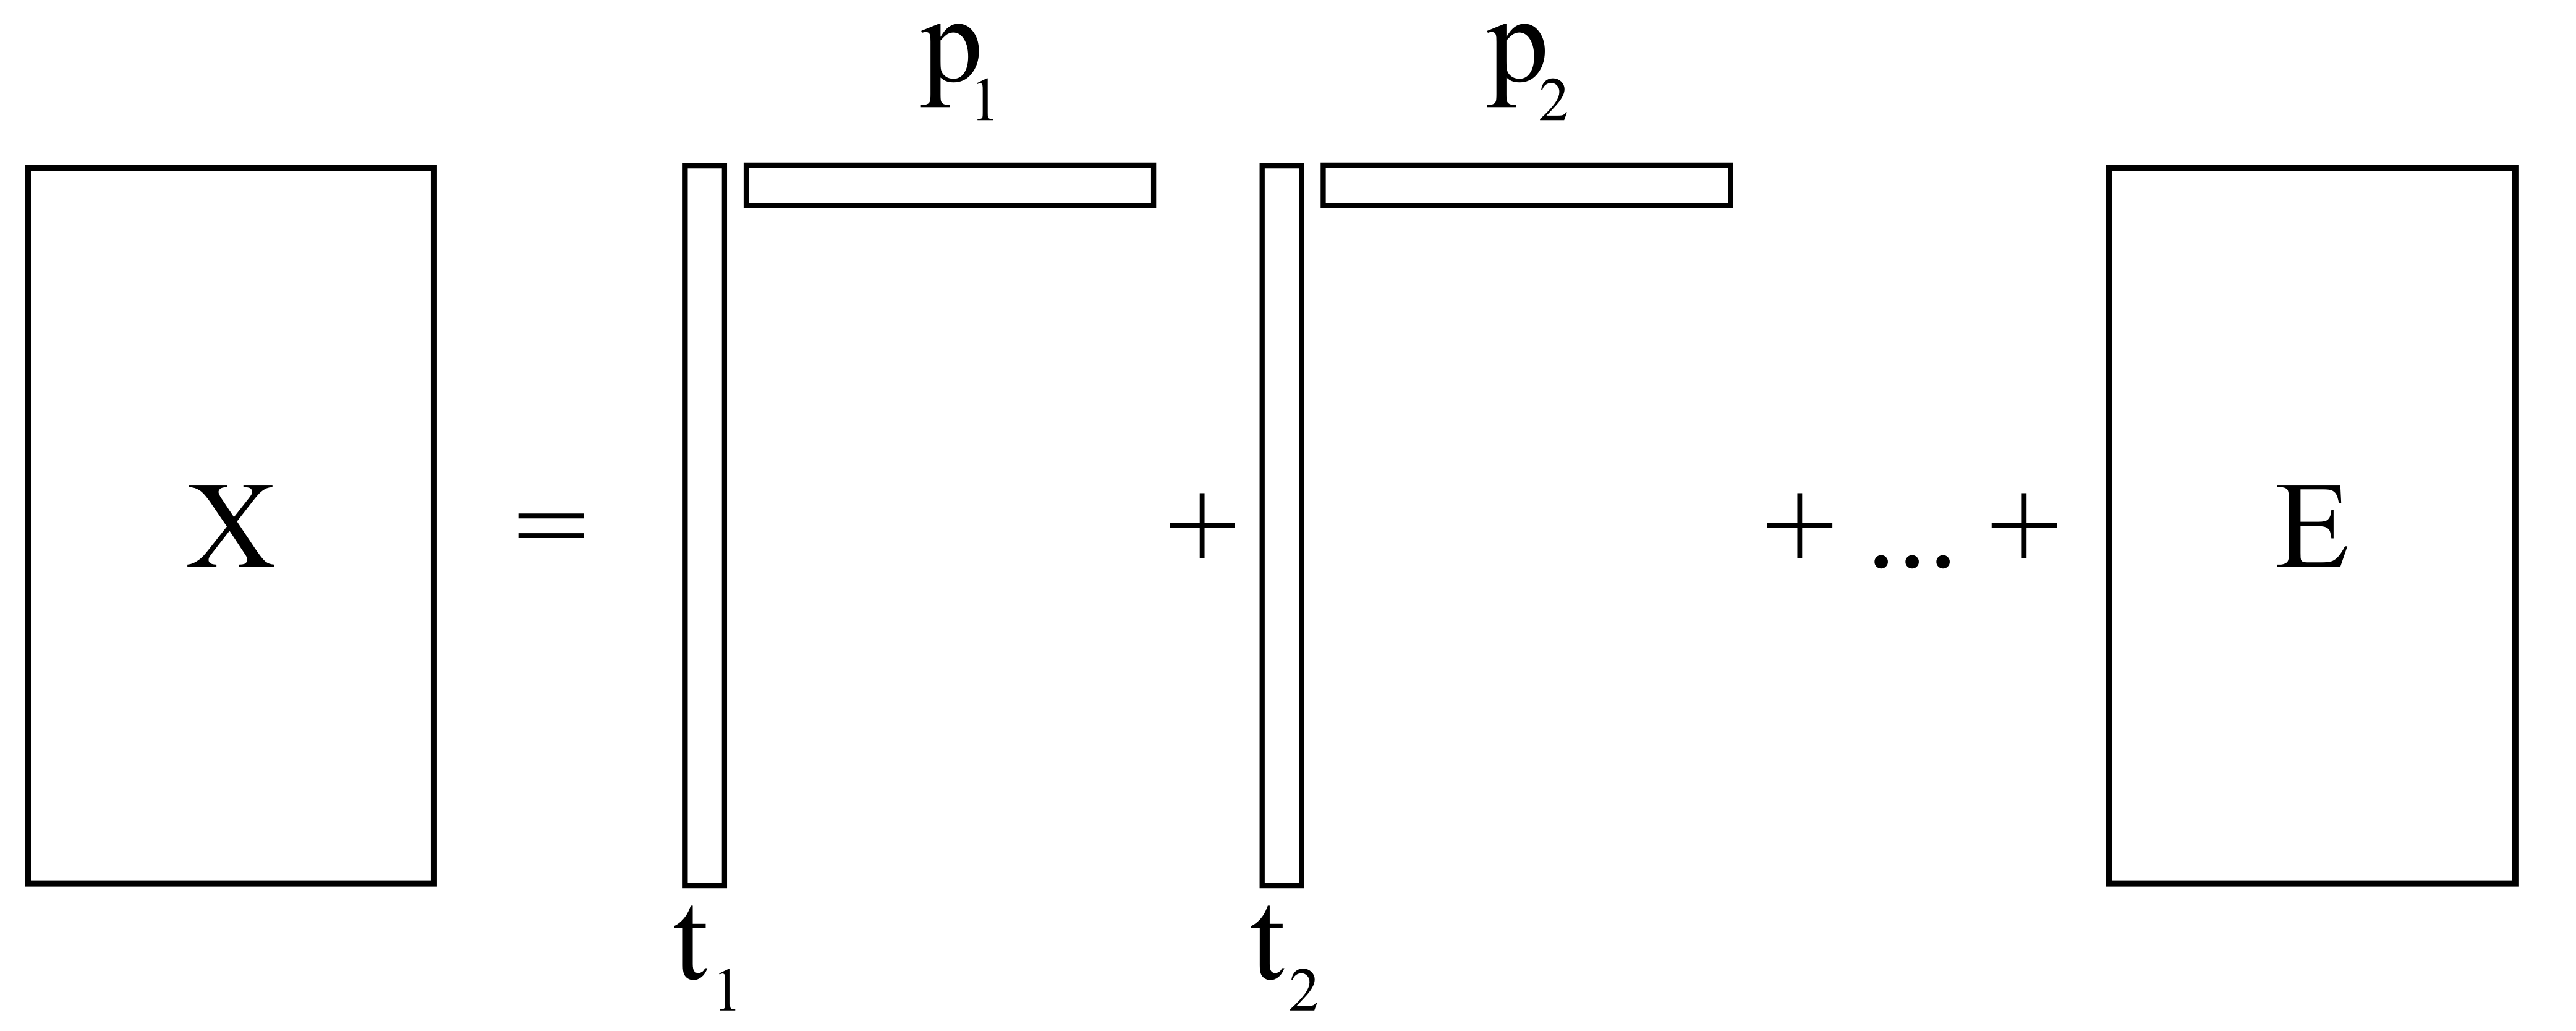
\includegraphics[height=0.5\textheight]{figures/pca_decomposition} \\
            {\scriptsize%
             From \textit{Process Improvement Using Data}}
        \end{center}}
    \only<3>{%
        \vspace{1em}
        \begin{center}
            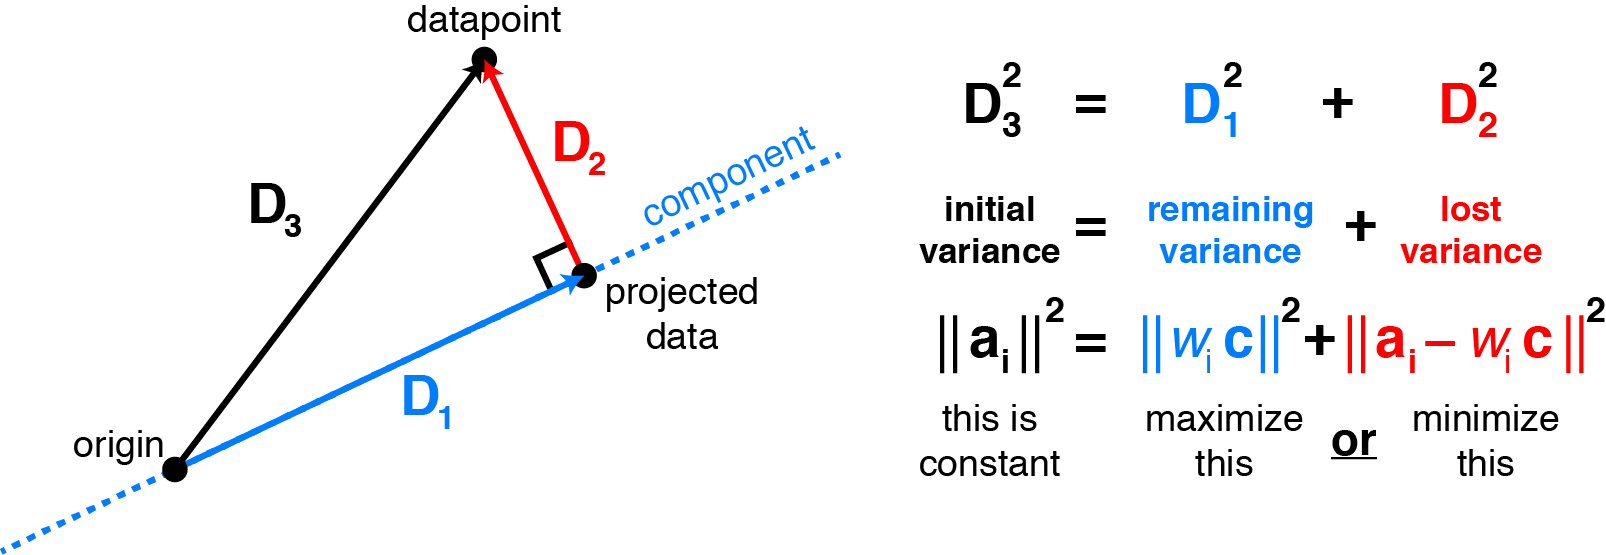
\includegraphics[width=\textwidth]{figures/pca_projection} \\[\bigskipamount]
            {\scriptsize%
             From Alex Williams' blog}
        \end{center}}
    \only<4>{%
        \vspace{1em}
        \begin{center}
            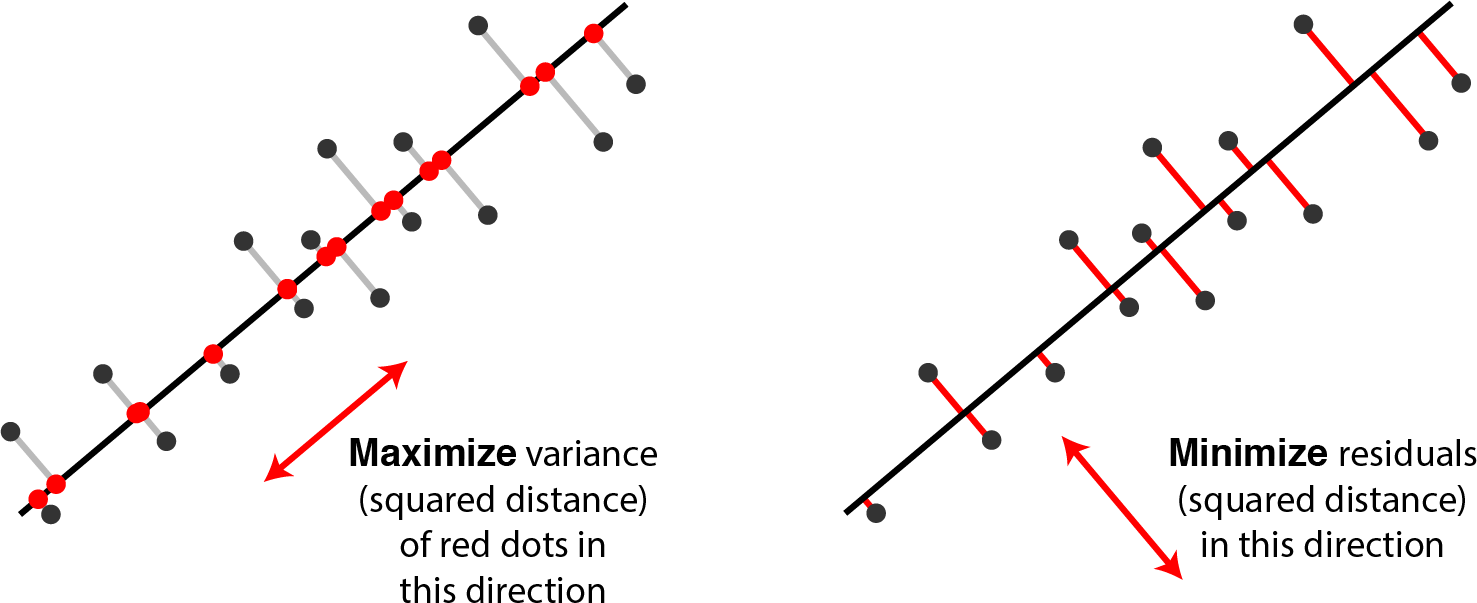
\includegraphics[width=\textwidth]{figures/pca_two_views} \\[\bigskipamount]
            {\scriptsize%
             From Alex Williams' blog}
        \end{center}}
\end{frame}

\begin{frame}{Partial least squares (PLS) regression}
    \only<1>{%
        \begin{center}
            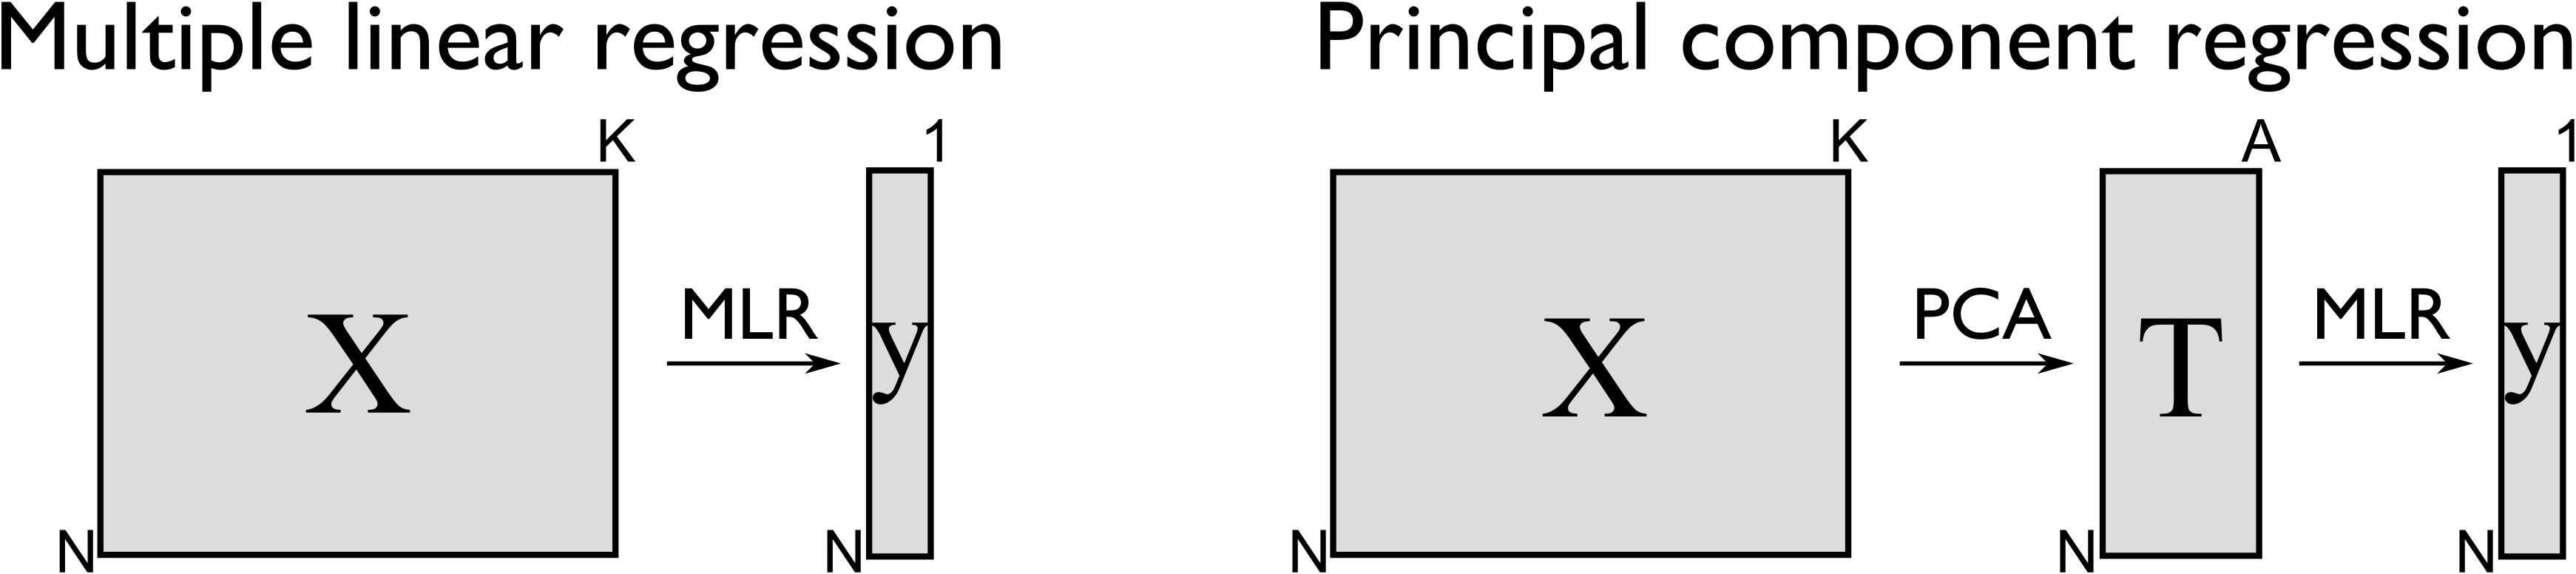
\includegraphics[width=\textwidth]{figures/lr_vs_pcr} \\
            {\scriptsize%
             From \textit{Process Improvement Using Data}}
        \end{center}
        \begin{block}{Advantages}\vspace{-0.5em}
            \begin{itemize}
                \item Single\hyp{}step model
                \item Components capture variability in $\mat{X}$ \alert{and}
                      $\mat{Y}$
                \item[$\rightarrow$] Fewer components, more compact model
            \end{itemize}
        \end{block}}
    \only<2>{%
        \begin{center}
            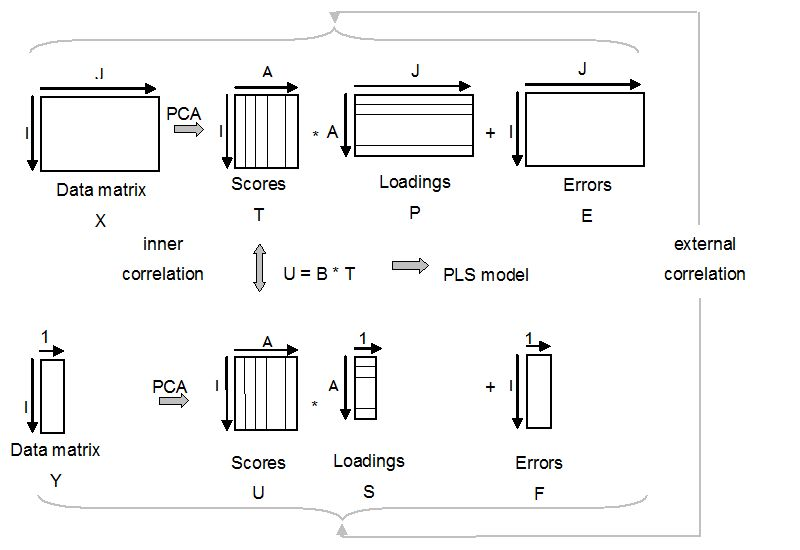
\includegraphics[height=0.8\textheight]{figures/pls} \\
            {\scriptsize%
             From Böhm et al.\ (2013)}
        \end{center}}
\end{frame}

\end{document}

